\documentclass[../bericht.tex]{subfiles}

\begin{document}

  \chapter{Einleitung}

    Die Sekunde ist das $9.192.631.770$-fache der Periodendauer der dem \"Ubergang zwischen den beiden Hyperfeinstrukturniveaus des Grundzustandes von Atomen des Nuklids $\mathrm{^{133}Cs}$ entsprechenden Strahlung - so die Definition nach dem SI-Einheitensystem. Genau diese Periodendauer soll im folgenden Versuch gemessen werden. Hierzu werden sowohl die Feinstruktur als auch die Hyperfeinstruktur erkl\"art und mittels der dopplerfreien Spektroskopie der \"Ubergang aufgel\"ost.


  \chapter{Versuch}

    \section{Feinstruktur}
    \label{sec:feinstruktur}

      Nach dem semiklassischen Atommodell kreisen die negativ geladenen Elektronen auf einer Kreisbahn um den positiv geladenen Atomkern. Die Rotation stellt einen Kreisstrom dar. Dieser erzeugt ein magnetisches Dipolmoment, welches \"uber den Bahndrehimpuls $\vec{l}$ ausgedr\"uckt werden kann. Gem\"a\ss dem \textsc{Stern-Gerlach}-Experiment (und anderen Experimenten) haben Elektronen ein weiteres magnetisches Dipolmoment inne, welchem der Spin $\vec{s}$ zugrunde liegt. Die beiden magnetischen Momente wechselwirken in der sogenannten \textit{Spin-Bahn-Kopplung}. Je nach Einstellung des Elektronenspins (\textit{Spin-up}/ \textit{Spin-down}, d.h. f\"ur die $z$-Komponente des Spins $s_z=\pm \frac{\hslash}{2}$) ergibt sich eine positive, bzw. negative Energiekorrektur $\Delta E_{l,s}$, die sogenannte \textit{Spin-Bahn-Kopplungsenergie}.

      Bei der mathematischen Betrachtung sind f\"ur die \textit{Feinstrukturaufspaltung} au\ss{}erdem relativistische Effekte zu beachten. Auf der Umlaufbahn um den ruhenden Kern dreht sich das Elektron einmal um die zum Drehimpuls parallele Achse. Dies f\"uhrt zu einer Korrektur der kinetischen Energie $\Delta E_\mathrm{rel}$.

      Zuletzt muss der \textit{\textsc{Darwin}-Term} $\Delta E_\mathrm{Darwin}$ ber\"ucksichtigt werden. Als Folge der relativistischen Zitterbewegung des Elektrons auf seiner Kreisbahn verkompliziert sich die elektrostatische Wechselwirkung zwischen Elektron und Atomkern.
      \medskip

      Die gesamte Energiekorrektur
      \begin{equation*}
        \Delta E = \Delta E_{l,s} + \Delta E_\mathrm{rel} + \Delta E_\mathrm{Darwin}
      \end{equation*}
      f\"uhrt zur sogenannten \textit{Feinstrukturaufspaltung}.
      \medskip

      Zur Beschreibung dieser Zust\"ande wird der Gesamtdrehimpuls $\vec{j}=\vec{l}+\vec{s}$ mit der zugeh\"origen gutartigen Gesamtdrehimpulsquantenzahl $j$ eingef\"uhrt. Letzte kann die Werte
      \begin{equation*}
        j=+\frac{1}{2} \quad\text{f\"ur}\quad l=0
      \end{equation*}
      und
      \begin{equation*}
        j=l\pm \frac{1}{2}\quad\text{f\"ur}\quad l>0
      \end{equation*}
      annehmen. Somit spalten alle Zust\"ande mit $l>0$ in zwei \textit{Feinstrukturniveaus} auf.


    \section{Hyperfeinstruktur}
    \label{sec:hyperfeinstruktur}

      Analog zum Spin des Elektrons wird auch dem r\"aumlich ausgedehnten Atomkern ein Spin zugeordnet, der sogenannte \textit{Kernspin} $\vec{I}$. Das dem Spin zugeordnete magnetische Moment des Kerns wechselwirkt mit dem Gesamtspin des Elektrons $\vec{j}$. Wiederum kommt es je nach Ausrichtung des Kernspins zu einer Energiekorrektur welche positiv und negativ ausfallen kann. Die Projektion auf die $z$-Richtung von $\vec{I}$ kann die $(2I + 1)$ Werte
      \begin{equation*}
        I_z=m_I \cdot \hslash\quad\text{mit}\quad -I\le m_I \le +I
      \end{equation*}
      annehmen. Zur Zustandsbeschreibung wird nun der Gesamtdrehimpuls des Atoms $\vec{F}=\vec{j}+\vec{I}$ mit der zugeh\"origen gutartigen Quantenzahl $F$,
      \begin{equation*}
        |j-I| \le F\le |j + I|
      \end{equation*}
      eingef\"uhrt. Die \textit{Feinstrukturniveaus} spalten also in
      \begin{equation*}
        \begin{cases}
            (2I+1), & I<j\\
            (2j+1), & j<I
        \end{cases}
      \end{equation*}
      \textit{Hyperfeinstrukturniveaus} auf. Aufgrund der im Vergleich zum Elektron extrem gro\ss{}en Masse des Kerns
      \begin{equation*}
        m_\mathrm{Kern}\approx Z\cdot 1836 \cdot m_\mathrm{e},
      \end{equation*}
      mit der Kernladungszahl $Z$, ist die Energieaufspaltung in Folge der \textit{Hyperfeinstruktur} sehr klein. Um diese zu messen ist also extrem schmalbandiges Licht notwendig, welches gleichzeitig so intensiv sein muss, dass ein messbares Signal entsteht. Weil Monochromatoren zu breitbandig sind, erfordert das Experiment also einen Laser.


    \section{Termschema von C\"asium}
    \label{sec:termschema-caesium}

      Im Versuch wird das Nuklid $\mathrm{^{133}Cs}$ verwendet. F\"ur die Zust\"ande wird die Nomenklatur $n^{2s+1}l_j$  verwendet. Der relevante Teil des Termschemas von C\"asium f\"ur den Versuch, d.h. der Grundzustand $\mathrm{6^2 S_{1/2}}$ und der angeregte Zustand $\mathrm{6^2P_{3/2}}$ mit Feinstrukturaufspaltung und Hyperfeinstrukturaufspaltung sind in \cref{fig:feinstruktur-hyperfeinstruktur} abgebildet. Die Kernspinquantenzahl ist $I=\frac{7}{2}$. Weiter sind die erlaubten angeregten optischen \"Uberg\"ange rot eingezeichnet. F\"ur diese ist zu beachten, dass anregende Photonen einen Spin von $1$ tragen. Bei Verwendung von linear polarisiertem Licht gelten die \"Ubergangsregeln
      \begin{equation*}
        \Delta l = 1\quad \text{und}\quad \Delta F = -1,0,+1.
      \end{equation*}

      \begin{figure}[tb]
        \centering
        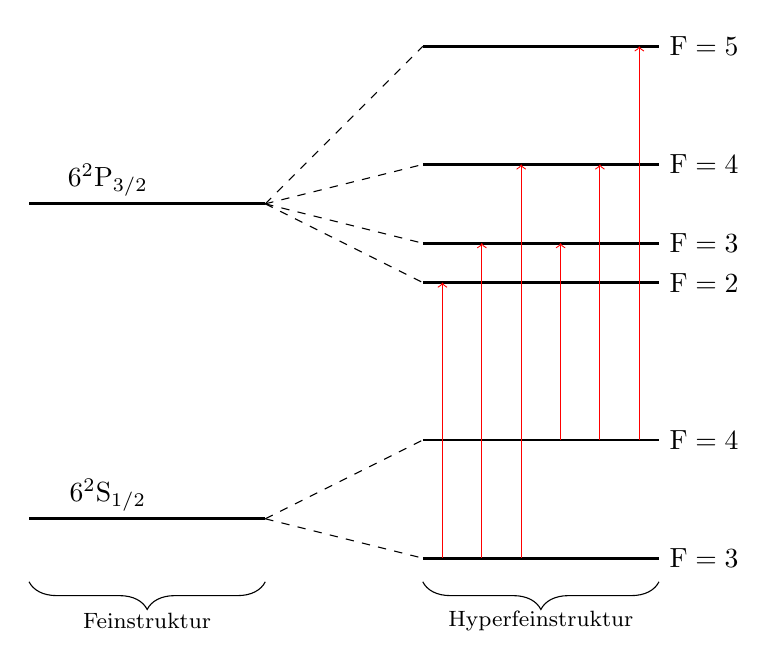
\begin{tikzpicture}
          % angeregte Niveaus
          \node at (1,4.3) {$\mathrm{6^2P_{3/2}}$};
          \draw[line width=1pt] (0,4)--(3,4);
          \draw[line width=1pt] (5,6)--(8,6) node[anchor=west] {$\mathrm{F=5}$};
          \draw[line width=1pt] (5,4.5)--(8,4.5) node[anchor=west] {$\mathrm{F=4}$};
          \draw[line width=1pt] (5,3.5)--(8,3.5) node[anchor=west] {$\mathrm{F=3}$};
          \draw[line width=1pt] (5,3)--(8,3) node[anchor=west] {$\mathrm{F=2}$};
          \draw[dashed] (3,4)--(5,6);
          \draw[dashed] (3,4)--(5,4.5);
          \draw[dashed] (3,4)--(5,3.5);
          \draw[dashed] (3,4)--(5,3);
          % Grundzustand Niveaus
          \node at (1,0.3) {$\mathrm{6^2S_{1/2}}$};
          \draw[line width=1pt](0,0)--(3,0);
          \draw[line width=1pt] (5,1)--(8,1) node[anchor=west] {$\mathrm{F=4}$};
          \draw[line width=1pt] (5,-0.5)--(8,-0.5) node[anchor=west] {$\mathrm{F=3}$};
          \draw[dashed] (3,0)--(5,1);
          \draw[dashed] (3,0)--(5,-0.5);
          % \"Uberg\"ange
          % Unterer Grundzustand
          \draw[color=red, ->] (5.25,-0.5)--(5.25,3);
          \draw[color=red, ->] (5.75,-0.5)--(5.75,3.5);
          \draw[color=red, ->] (6.25,-0.5)--(6.25,4.5);
          % Oberer Grundzustand
          \draw[color=red, ->] (6.75,1)--(6.75,3.5);
          \draw[color=red, ->] (7.25,1)--(7.25,4.5);
          \draw[color=red, ->] (7.75,1)--(7.75,6);
          % Fein- und Hyperfeinstruktur
          \draw [decorate,decoration={brace,mirror,amplitude=10pt}] (0,-0.8) -- (3,-0.8) node [black,midway,yshift=-14pt] {\footnotesize Feinstruktur};
          \draw [decorate,decoration={brace,mirror,amplitude=10pt}] (5,-0.8) -- (8,-0.8) node [black,midway,yshift=-14pt] {\footnotesize Hyperfeinstruktur};
        \end{tikzpicture}
        \caption{Termschema von $\mathrm{^{133}Cs}$ ($I=\frac{7}{2}$) mit Feinstruktur und Hyperfeinstruktur. Die erlaubten Anregungs\"uberg\"ange sind rot markiert. }
        \label{fig:feinstruktur-hyperfeinstruktur}
      \end{figure}


    \section{Diodenlaser}
    \label{sec:diodenlaser}

      Es folgt eine Kurzfassung von ??? zur Funktion von Diodenlasern.

      Diodenlaser sind aus Halbleitern aufgebaut. Bei der Rekombination von Elektronen im Leitungsband mit den L\"ochern im Valenzband wird das Laserlicht emittiert. Der Hauptteil eines Diodenlasers besteht aus einem $p-n$-\"Ubergang, welcher durch Dotierung erzeugt wird. Die Besetzungsinversion mit L\"ochern im Valenzband und Elektronen im Leitungsband wird durch das Anlegen einer Spannung erreicht. Dieser Prozess ist der Pumpprozess des Lasers. Die Rekombination der L\"ocher und Elektronen kann spontan oder stimuliert erfolgen. Das dabei emittierte Licht ist nur koh\"arent, falls die stimulierte Emission \"uberwiegt. Aufgrund des hohen Brechungsindexes $n$ der Halbleiterkristalle betr\"agt die Reflektivit\"at der Grenzfl\"ache zu Vakuum in etwa $\SI{30}{\percent}$. Damit k\"onnen die Kristalle selbst, ohne weitere Behandlung, als Resonatoren fungieren. Diejenige Seite, auf der kein Licht austreten soll, wird zus\"atzlich verspiegelt. F\"ur die Ausbildung von stehenden Wellen im Resonator gilt der Zusammenhang
      \begin{equation*}
        \lambda = \frac{2nL}{m}.
      \end{equation*}
      Hierbei ist $\lambda$ die Wellenl\"ange des Lichts, $L$ die L\"ange des Resonators (Halbleiterkristalls) und $m$ eine nat\"urliche Zahl.

      Einer der Vorteile eines Diodenlasers ist dessen Durchstimmbarkeit bez\"uglich der Frequenzen. In Abh\"angigkeit der Betriebstemperatur $T$ und der Stromst\"arke $I$ ??? \"andert sich die Frequenz der Laserstrahlung. Die Temperatur beeinflusst die Ausdehnung des Kristalls und damit die L\"ange des Resonators. Unter Voraussetzung einer konstanten Temperatur \"andert sich mit der Stromst\"arke die Ladungstr\"agerdichte im Halbleiter. Damit \"andert sich auch der Brechungsindex des Kristalls und somit die optische L\"ange des Resonators.
      Die Durchstimmbarkeit ist f\"ur diesen Versuch von Bedeutung, um die Resonanzfrequenz von C\"asium zu treffen.
      \medskip

      Weiter weist ein Diodenlaser, wie alle Laser, eine schmale Linienbreite auf, welche n\"otig ist um die Energieaufspaltung der Hyperfeinstruktur aufl\"osen zu k\"onnen. Das Spektrum des verwendeten Lasers ist in ??? abgebildet. Dieses ist jedoch noch immer zu breit f\"ur die gew\"unschte Aufl\"osung der Hyperfeinstruktur. Die Linienbreite des Lasers erscheint verbreitert durch die \textit{nat\"urliche Linienbreite}, \textit{\textsc{Doppler}verbreiterung} und \textit{Druckverbreiterung}. Dominant ist hierbei die \textit{\textsc{Doppler}verbreiterung}, wie in folgenden Abschnitten erl\"autert wird. Deshalb folgt auch die Notwendigkeit der \textit{\textsc{doppler}freien Spektroskopie} (vgl. \ref{sec:dopplerfreie-spektroskopie}).
      \medskip

      Der in diesem Versuch verwendete Diodenlaser weist den in \cref{fig:laserschwelle} abgebildeten Zusammenhang zwischen Eingansstrom und Ausgangsleistung auf. Die lineare Regression f\"ur Messpunkte mit Eingangsstrom $I\ge 31$ liefert die Gerade
      \begin{equation}
        P(I)=-\SI{5,21(6)}{\milli\watt} + \SI{0,156(1)}{\volt}\cdot I
        \label{eq:laserschwellen-plot}
      \end{equation}
      Und damit die Laserschwelle
      \begin{equation}
        I_\mathrm{Schwelle}=\SI{33,37(56)}{\ampere}.
        \label{eq:laserschwelle}
      \end{equation}
      Gemessen wurde die Ausgangsleistung in Abh\"angigkeit des \textit{Coarse} der Spannungsquelle. Mithilfe von \textit{Coarse}-Stromst\"arke-Kennlinie des Netzteils des Diodenlasers (\cref{sec:netzteil-kennlinie}) wird die Eingangsstromst\"arke des Lasers ermittelt. Diese Daten liegen nicht in digitaler Form vor und mussten deshalb vom Graphen abgelesen werden. Hierbei ist ein nicht zu vernachl\"assigender Fehler aufgetreten, der, zusammen mit dem unbekannten Fehler der des Graphen selber, auf
      \begin{equation*}
        \delta I = \pm \SI{2}{\milli\ampere}
      \end{equation*}
      gesch\"atzt wird. Zudem liegt der Fehler des Powermeters??? bei
      \begin{equation*}
        \delta P = 0,003 \cdot P.
      \end{equation*}
      Beide Fehler sind mithilfe der Fehlerbalken in \cref{fig:laserschwelle} angegeben. Bei der Berechnung der Laserschwelle wurde der Fehler des Powermeters mit einer $\frac{1}{Fehler}$-Gewichtung ber\"ucksichtigt. Die Messungen wurden bei der Diodenlasertemperatur
      \begin{equation*}
        T=\SI{21,4(20)}{\celsius}
      \end{equation*}
      durchgef\"uhrt. W\"ahrend die Anzeige des Regelungsinstruments den Wert laut technischer Daten pr\"aziser angibt, ist das Ger\"at seit Jahren nicht geeicht geworden. Deshalb dient die Anzeige nur als Anhaltspunkt, bzw. f\"ur Temperaturdifferenzen, jedoch nicht f\"ur absolute Temperaturmessungen. Dmeentsprechen gro\ss{} ist der Fehler mit $\SI{2}{\celsius}$  gew\"ahlt.

      \begin{figure}[tb]
        \begin{tikzpicture}
            \def\Imin{0}
    				\def\Imax{100}
    				\def\Pmin{0}
    				\def\Pmax{10}eq:laserschwelle
            %
            \begin{axis}[
              /tikz/line join=bevel,
              width=0.8*\textwidth,
              height=0.5*\textwidth,
              grid,
              legend style={at={(0,1)}, legend columns=1, anchor=north west},
              every axis plot,
    					xmin = \Imin, xmax = \Imax,
    					ymin = \Pmin, ymax = \Pmax,
    					xlabel = {Eingangsstrom $I$ in $\si{\milli\ampere}$},
    					ylabel = {Laserleistung $P$ in $\si{\milli\watt}$},
              ]
    					% Add plots
    					\addplot[only marks, color=blue, line width = 1pt] plot [error bars/.cd, y dir = both, y explicit, x dir = both, x explicit] table [x=current,y=power, x error=current-error, y error=power-error]{data/laser_threshold.txt};
    					\addlegendentry{Messpunkte}
    					\addplot[draw=red, line width = 1pt][domain=30:100]{-5.21048967 + 0.15615788 * x};
    					\addlegendentry{Lineare Regression}
            \end{axis}
        \end{tikzpicture}
        \caption{Ausgangsleistung $P$ als Funktion des Eingangsstroms $I$ der verwendeten Laserdiode bei einer Temperatur von $T=\SI{21,4(20)}{\celsius}$. Eingezeichnet ist auch die lineare Regression \cref{eq:laserschwellen-plot} zur Bestimmung der Laserschwelle \cref{eq:laserschwelle}.}
        \label{fig:laserschwelle}
      \end{figure}


      \subsection{Druckverbreiterung}
      \label{subsec:druckverbreiterung}

        Je nach Gasdruck in der Gaskammer kommt es zu mehr oder weniger St\"o\ss{}en zwischen den
        C\"asium-Atomen. Die Wechselwirkung zwischen den Atomen beeinflusst das Termschema und
        verbreitert damit die Spektrallinien. Die Linienverbreiterung ist proportional zum Druck. Somit kann und wird der Effekt der \textit{Druckverbreiterung} durch einen kleinen Druck in der Gaskammer minimiert.


      \subsection{Nat\"urliche Linienbreite}
      \label{subsec:natueliche-linienbreite}

        Angeregte Zust\"ande haben nur eine endliche Lebensdauer bevor das System wieder in den Grundzustand relaxiert. Nach der \textit{\textsc{Heisenberg}'schen Unsch\"arferelation} k\"onnen Zeit und Energie aber nicht gleichzeitig scharf bestimmt werden. Somit geh\"oren zu Zust\"anden mit begrenzter Lebensdauer unscharfe Energieniveaus. Dies sorgt f\"ur eine Verbreiterung der Spektrallinien. Die Unsch\"arfe aufgrund der sogenannten \textit{nat\"urlichen Linienbreite} ist allerdings f\"ur die optischen C\"asium \"Uberg\"ange, welche in diesem Versuch von Interesse sind, hinreichend klein um die Hyperfeinstruktur aufl\"osen zu k\"onnen.


      \subsection{Dopplerverbreiterung}
      \label{subsec:dopplerverbreiterung}

        Gem\"a\ss dem relativistischen \textsc{Doppler}-Effekt \"andert sich die Frequenz eines einfallenden Photons im Ruhesystem eines (C\"asium-) Atoms, falls das Atom eine Geschwindigkeitskomponente ungleich Null parallel zur Bahn des Photons aufweist. Im Falle von entgegengesetzten Bewegungen von Atom und Photon kommt es zur Blauverschiebung (die vom Atom observierte Frequenz wird gr\"o\ss{}er), im Falle von gleichgerichteten Bewegungen zur Rotverschiebung (die vom Atom observierte Frequenz wird kleiner). Mit dem \textsc{Doppler}-Effekt als Ursache wird diese Linienverbreiterung \textit{\textsc{Doppler}verbreiterung} genannt.


    \section{Transmissionsspektroskopie}
    \label{sec:transmissionsspektroskopie}




    \section{Dopplerfreie Spektroskopie}
    \label{sec:dopplerfreie-spektroskopie}


      6 statt 3 erwartete Peaks


      \subsection{Cross-over Resonanzen}
      \label{subsec:cross-over-resonanzen}

        genau in der mittels


    \section{Zeeman-Effekt}
    \label{sec:zeeman-effekt}

      nicht observierbar!










\end{document}
